\documentclass[UTF8,10pt,fontset=none]{ctexart}
\setCJKmainfont[Path=C:/Windows/Fonts/,BoldFont=simhei.ttf,ItalicFont=simkai.ttf]{simsun.ttc}
\setCJKsansfont[Path=C:/Windows/Fonts/]{simhei.ttf}
\setCJKmonofont[Path=C:/Windows/Fonts/]{simfang.ttf}
\setCJKfamilyfont{zhsong}[Path=C:/Windows/Fonts/,BoldFont=simhei.ttf]{simsun.ttc}
\setCJKfamilyfont{zhhei}[Path=C:/Windows/Fonts/]{simhei.ttf}
\setCJKfamilyfont{zhfs}[Path=C:/Windows/Fonts/]{simfang.ttf}
\setCJKfamilyfont{zhkai}[Path=C:/Windows/Fonts/]{simkai.ttf}
\usepackage[a4paper,left=24mm,right=24mm,top=24mm,bottom=24mm]{geometry}
\usepackage{booktabs,amsmath,amssymb,amsthm}
\usepackage{algorithm,algpseudocode,graphicx,subcaption}
\usepackage{longtable,array}
\usepackage[round,authoryear]{natbib}
\usepackage[hidelinks]{hyperref}
\usepackage{url}
\usepackage[section]{placeins}
\hypersetup{pdftitle={机制分歧驱动的主动证据选择与集合校准：面向组合式多智能体社会模拟},pdfauthor={研究论文中文全文}}
\newtheorem{proposition}{命题}
\renewcommand{\proofname}{证明}
\floatname{algorithm}{算法}
\algrenewcommand\algorithmicrequire{\textbf{输入：}}
\algrenewcommand\algorithmicreturn{\textbf{输出}}
\algrenewcommand\algorithmicif{\textbf{若}}
\algrenewcommand\algorithmicthen{\textbf{则}}
\algrenewcommand\algorithmicelse{\textbf{否则}}
\algrenewcommand\algorithmicend{\textbf{结束}}
\algrenewcommand\algorithmicfor{\textbf{对}}
\algrenewcommand\algorithmicdo{\textbf{执行}}
\algrenewcommand\algorithmicwhile{\textbf{当}}
\newcommand{\E}{\mathbb{E}}
\newcommand{\R}{\mathbb{R}}
\newcommand{\ind}{\mathbf{1}}
\DeclareMathOperator{\Var}{Var}
\DeclareMathOperator{\Cov}{Cov}
\DeclareMathOperator{\tr}{tr}
\DeclareMathOperator*{\argmax}{arg\,max}
\setlength{\parskip}{3pt}
\setlength{\textfloatsep}{12pt plus 2pt minus 2pt}
\emergencystretch=2em
\graphicspath{{figures_zh/}}
\newcommand{\DevReduction}{78.94}
\newcommand{\InitialDev}{0.025791}
\newcommand{\FinalDev}{0.005432}
\newcommand{\TestAUC}{0.006916}
\newcommand{\FrozenSpeed}{217.95}
\newcommand{\UniformSpeed}{275.16}
\newcommand{\ESS}{1.000385}
\newcommand{\MaxWeight}{0.999808}
\newcommand{\MacroFull}{0.007064}
\newcommand{\MacroRandom}{0.007059}
\newcommand{\MacroMAP}{0.007065}
\newcommand{\DevBrierStart}{0.189335}
\newcommand{\DevBrierEnd}{0.242053}
\newcommand{\TestBrier}{0.245921}
\newcommand{\TestCoverage}{97.92}
\newcommand{\TestWidth}{0.030382}
\newcommand{\TestRuntime}{7.69}
\newcommand{\TestVRAM}{14.59}
\newcommand{\HistoryPair}{0.011732}
\newcommand{\ProbePair}{0.011481}

\title{机制分歧驱动的主动证据选择与集合校准\\面向组合式多智能体社会模拟}
\author{研究论文中文全文}
\date{}
\begin{document}
\maketitle
\begin{abstract}
拟合历史参与总量，并不意味着识别了产生这些总量的行为机制。广泛的信息触达与较低的参与意愿，以及有限的信息触达与较高的参与意愿，都可能解释同一段历史；但在候补、同伴转发和时间冲突共同作用时，两者可能给出不同预测。本文研究这一情境下的预算化过程证据获取。我们保留有限个与历史相容的模拟机制，分别依据过程记录和群体轨迹筛选跨活动共享的阶段参数，再按噪声归一化的最差活动误差分配权重。缓存的组合探针把预期预测方差缩减转化为加权协方差计算，小批量查询通过对假设结果求期望完成条件化，无需重新运行模拟器。在 V1 可审计的 60 候选开发搜索中，归一化轨迹误差 AUC 下降 \DevReduction\%，冻结合成测试 AUC 为 \TestAUC；GPU 配对微基准显示，协方差评分比所提供的显式枚举实现快 \FrozenSpeed\ 倍。然而，24 个独立合成世界的评测揭示了一个重要限制：所选校准分布的有效机制数只有 \ESS，同先验取证、匹配单点估计以及两项取证消融的表现几乎一致，未知规则诊断也会漏检较弱偏移。这些结果给出了高效、可复现的实现，同时表明：群体预测的改善，可能压缩主动取证所依赖的机制分歧。另行开展的 30 配置扩展保留了非坍缩先验，在构造交互压力测试上恢复了同先验取证增益，但与参数信息增益持平。本文仅提供合成证据，不主张真实数据成效、官方榜单排名或一般性的次模保证。
\end{abstract}

\section{引言}
假设两个模拟系统预测某项活动的到场人数相同。第一个系统中，几乎所有人都收到通知，但感兴趣的人很少；第二个系统中，收到通知的人很少，但这些人大多愿意参加。仅凭历史到场人数，无法区分两种解释。当新活动同时涉及消息转发、候补名单和日程重叠时，这种区别就会影响结果：转发决定哪些人知道机会，候补流转决定谁能获得名额，冲突则决定哪些参与意图最终转化为实际到场。这个例子同样适用于更广泛的资源分配与集体参与过程。校园是一个可执行实例，并不是研究问题的应用边界。

因此，从群体输出反推机制，是一个可能不可识别的逆问题。已有集合校准研究已经承认，多个参数配置可以同时满足统计上的相容要求 \citep{bai2022}。接下来的实际问题是：当逐条收集微观记录没有必要或代价过高时，应该补充哪一条过程观测？某条记录的行为熵很高，却可能对未来关心的预测几乎没有帮助。反过来，对于“是否查看过通知”的一个不大的分歧，如果能够区分未来拥挤轨迹不同的机制，就可能很有价值。目标导向实验设计提供了相应视角：证据价值取决于它要改善什么预测 \citep{chaloner1995,attia2018,zhong2026}。

本文用有限机制库、明确的环境结算和缓存化组合探针实现这一思路。共享参数控制注意、参与和候补退出；过程与轨迹分别接受相容性检查，形成候选集合。随后，轨迹加权规则定义一个校准混合分布，加权协方差按照“单位成本下预期减少多少探针预测分歧”对二元过程记录排序。同一缓存还支持后验更新与完整轨迹分布预测，查询步骤内部不需要重新训练模型或重跑模拟器。

实际结果比这一方法设计所暗示的更为有限。开发集选择强烈偏好集中的轨迹权重。最优预测器虽然在硬相容集合中保留了许多候选，但有效混合多样性几乎消失；轨迹分数改善的同时，个体过程的 Brier 分数却变差了。由于剩余可消除的机制分歧很小，取证消融的影响也不明显。这一现象揭示了一个直接影响方法有效性的张力：优化群体预测准确性，与为后续取证保留有用的不确定性，未必是同一个目标。

本文的贡献有三个方面。第一，针对严格区分行为意图与实际结果的多智能体模拟器，明确给出过程约束下的集合校准与预算化证据选择形式，并提供可复现实现。第二，将二元预测方差恒等式实现为批量协方差运算，在小批量中对假设标签积分，并说明计算与统计假设。我们不把该恒等式或目标导向设计原则本身当作新的理论贡献。第三，给出经过审计的合成研究，用同先验对照、逐活动不确定性和未知规则压力测试，区分校准收益与取证收益。结果表明，权重集中是一个实际失效模式，也约束了仅凭较好群体分数可以作出的推断。

本文应被理解为一项方法与诊断研究。它既没有证明在 SocioVerse 上达到当前最优，也没有取得 MIT 真实行为基准成绩。具有指定字段的接口不等于已经评测了相应数据集。一般数学形式可以迁移，但当前经验结论只针对这里的构造系统。

\section{问题定义}
\label{sec:setup}
\paragraph{部分可观测的社会动态。}
用 $i\in\{1,\ldots,N\}$ 表示智能体，$e$ 表示活动。时刻 $t$ 的全局状态为 $s_t=(h_{1t},\ldots,h_{Nt},g_t)$。其中，$h_{it}$ 包含兴趣、可用时间、剩余预算、已收信息和参与经历；环境状态 $g_t$ 包含通知、报名窗口、容量、报名结果、候补名单与日程。智能体获得局部观测 $o_{it}\sim O_i(\cdot\mid s_t)$，并形成意图 $u_{it}\sim\pi_\theta(\cdot\mid o_{it},h_{it})$。社会互动产生消息 $m_t\sim G_\theta(\cdot\mid s_t,u_t)$。环境把意图与消息结算为实际行动结果，再反馈到状态：
\begin{equation}
 a_t\sim K_\xi(\cdot\mid s_t,u_t,m_t),\qquad
 s_{t+1}\sim F_\xi(\cdot\mid s_t,a_t,m_t).
 \label{eq:loop}
\end{equation}
$\xi$ 表示环境规则。式~\eqref{eq:loop} 描述一个部分可观测的多智能体随机系统，并不要求额外声称它进行了奖励优化或策略学习。想报名不等于报名成功：容量、时间冲突和预算可能使意图无法兑现，取消与递补也会改变后续参与结果。

实现中的 $\theta=(a,b,d)$ 分别控制注意、条件参与和候补退出，在不同活动之间共享。个体状态和活动特征仍然不同，因此个体概率也不同。每个模拟世界中，同一批人参与相互影响的活动。群体轨迹 $X_{etc}$ 记录报名、候补和到场比例，$c\in\{1,2,3\}$ 表示三个通道。对候选 $m$ 与种子 $s$，缓存轨迹记为 $X_{msetc}$。每条轨迹全程使用同一个机制；平均参数或在时间步间切换机制，会定义另一个不同的模拟器。

\paragraph{历史信息与取证机会。}
历史数据包括观测轨迹，以及来自独立核查人群的二元阶段记录。取证池由另外一批人组成，每人只在一个标准化、机会状态已知的情境下贡献一条记录。候选概率为 $p_{mr}=P(Y_r=1\mid\theta_m,x_r)$，获取成本为 $k_r>0$。在本基准中，给定机制后各记录条件独立，记录是否可获取的元数据在查询前已知。我们不据此推断任意互动人群日志都相互独立。如果观察了组成记录，又把同一过程的汇总人数当成独立证据，就会重复计数；分离人群避免了这一特定依赖。

\paragraph{组合预测目标。}
活动配置记为 $\xi=(\ell,f,c,\eta)$，其中 $(\ell,f,c)$ 为候补、转发和冲突开关，$\eta$ 为其余属性。历史活动分别启用候补和转发；冲突规则存在于模拟器中，但所有历史配置均未启用。固定探针组合这些可访问规则，用于近似未来预测需求。取证策略 $\alpha$ 选择序列 $Q$，满足 $\sum_{r\in Q}k_r\leq B$，并更新机制混合分布。科学目标是在目标活动分布下获得较低的轨迹风险：
\begin{equation}
 \mathcal R_B(\alpha)=\E_{\xi,Y,Q\sim\alpha}\!\left[
 L\big(\widehat X(\xi\mid Y_Q),X^{\mathrm{true}}(\xi)\big)\right].
 \label{eq:risk}
\end{equation}
探针分歧是该风险的模型内部、可计算替代目标，并不保证是其无偏估计。缓存分为训练、探针、开发和测试库。开发阶段已包含成对和三重规则组合，测试采用不同活动实例，而不是整个开发阶段都未见过的组合。因此，本文研究的是超出经验训练活动的迁移，而非不受限制的组合分布外泛化。引入所有候选都没有的规则，则属于另一个模型失配实验。

\section{方法}
\label{sec:method}
以下公式对应冻结 V1 代码实际执行的分支；另行预注册的 V2 扩展见第~\ref{sec:round2} 节。最终演化改变的是校准距离，而不是协方差取证公式。源码中仍然保留但未启用的其他损失，不属于本文报告的方法。

\subsection{相容机制与校准权重}
设 $\bar X_{metc}=S^{-1}\sum_sX_{msetc}$，$H_{etc}$ 为历史观测的平均轨迹。对已观测历史记录 $\mathcal O$，分别定义过程与轨迹误差：
\begin{align}
 B_m&=|\mathcal O|^{-1}\sum_{r\in\mathcal O}(p_{mr}-y_r)^2,\nonumber\\
 R_m&=\left[(ETC)^{-1}\sum_{etc}(\bar X_{metc}-H_{etc})^2\right]^{1/2}.
 \label{eq:compaterrors}
\end{align}
当 $\mathcal O$ 为空时，令 $B_m=0$。相容集合为
\begin{equation}
 \mathcal C=\{m:B_m\leq\min_j B_j+0.045\}\cap\{m:R_m\leq0.10\}.
 \label{eq:set}
\end{equation}
集合为空时直接报错，而不是自动放宽阈值。这些经验筛选标准没有置信集合覆盖保证，也不保证真实机制位于候选网格内。过程 Brier 误差在这里是筛选统计量，不是伯努利对数似然。

最终校准规则用估计的模拟噪声归一化轨迹残差，并强调拟合最差的历史活动：
\begin{align}
 v_{etc}&=\frac1{MS}\sum_{m,s}(X_{msetc}-\bar X_{metc})^2,
 &\bar v&=\frac1{ETC}\sum_{etc}v_{etc},\nonumber\\
 r_{etc}&=\frac{v_{etc}+\epsilon}{\bar v+\epsilon},
 &D_m&=\max_e\frac1{TC}\sum_{tc}\frac{(\bar X_{metc}-H_{etc})^2}{r_{etc}},\label{eq:distance}\\
 w_m^{(0)}&=\frac{\ind\{m\in\mathcal C\}\exp[-D_m/(2\sigma^2)]}
 {\sum_{j\in\mathcal C}\exp[-D_j/(2\sigma^2)]},
 &\epsilon&=10^{-5},\quad\sigma=7\times10^{-4}.\label{eq:weights}
\end{align}
方差除数为 $S$，并在筛选前对全部 $M$ 个候选平均。这是种子方差，不是蒙特卡洛均值的方差。$r_{etc}$ 因而提供随时段和通道变化的精度权重；实现中没有另行学习的时间注意力项，也没有高阶取证修正项。所得分布是 Gibbs 型校准混合分布。若要称其为历史轨迹生成过程的精确后验，还需要一个实现中并未指定的观测似然。

\subsection{查看记录缺失与观测似然}
在标准化核查人群中，未观测的查看状态被积分消去。若 $V_r$ 表示是否查看，$I_r$ 表示参与意图，则
\begin{equation}
 P(I_r=1\mid\theta_m)=P(V_r=1\mid\theta_m)P(I_r=1\mid V_r=1,\theta_m)
 =a_m\rho_{e(r)}b_m\iota_r,
 \label{eq:view}
\end{equation}
其中 $\rho_e$ 是通知触达率，$\iota_r$ 是记录中的兴趣。因此，缺失查看不等于未查看。候补退出记录以已知候补风险状态为条件。这些公式不能替代对未知互动历史进行潜状态过滤。

对已经请求获取的记录，用 $o_r$ 表示结果是否被观测。本基准采用完全随机缺失（MCAR）：$o_r=1$ 时，$\ell_{mr}=p_{mr}^{y_r}(1-p_{mr})^{1-y_r}$；否则 $\ell_{mr}=1$。若提供已知观察模型 $\gamma_{mry}=P(o_r=1\mid Y_r=y,\theta_m)$，则使用
\begin{equation}
 \ell_{mr}=\begin{cases}
 p_{mr}^{y_r}(1-p_{mr})^{1-y_r}\gamma_{mr y_r},&o_r=1,\\
 (1-p_{mr})(1-\gamma_{mr0})+p_{mr}(1-\gamma_{mr1}),&o_r=0.
 \end{cases}
 \label{eq:missing}
\end{equation}
这一处理反映了对不可忽略观察过程进行建模的必要性 \citep{rubin1976}。可选分支通过了单元测试，但没有在真实缺失情境下得到验证。右删失则是另一类问题：尚未结束的事件时间观测需要例如 $P(T_r>t_{\mathrm{cut}}\mid\theta_m)$ 的生存似然，以及明确的事件时间模型。该扩展尚未实现；当前证据池仅包含观察机会已完整结束的二元记录。

\subsection{缓存探针与协方差取证恒等式}
令 $z_m\in\R^D$ 为候选在固定组合探针上的平均轨迹拼接向量，其中 $D=E_{\mathrm p}TC$。给定当前权重 $w$，定义
\begin{equation}
 \mu=\sum_mw_mz_m,\qquad q_r=\sum_mw_mp_{mr},\qquad
 c_r=\sum_mw_m(p_{mr}-q_r)(z_m-\mu).
 \label{eq:cov}
\end{equation}
取证价值为
\begin{equation}
 A_r(w)=\frac{\|c_r\|_2^2}{Dk_rq_r(1-q_r)},\qquad
 C=P^\top\operatorname{diag}(w)(Z-\mathbf1\mu^\top).
 \label{eq:score}
\end{equation}
$C$ 的各行包含所有 $c_r^\top$。矩阵乘法在记录之间共享计算。代码对 $q_r(1-q_r)$ 设置 $10^{-12}$ 的下限；确定性观测的精确理论价值为零。

\begin{proposition}[二元观测的预测方差缩减]
给定固定缓存条件均值 $Z=z_\theta$、模型隐含的二元观测分布以及 $0<q_r<1$，观测 $Y_r$ 后，平均坐标方差的预期减少量等于 $k_rA_r(w)$。
\end{proposition}
\begin{proof}
令 $\mu_y=\E[Z\mid Y_r=y]$。由贝叶斯公式，$\mu_1-\mu=c_r/q_r$，$\mu_0-\mu=-c_r/(1-q_r)$。利用全协方差分解，得到
\begin{align}
 \frac1D\tr\{\Cov(Z)-\E_{Y_r}\Cov(Z\mid Y_r)\}
 &=\frac{q_r\|\mu_1-\mu\|^2+(1-q_r)\|\mu_0-\mu\|^2}{D}\nonumber\\
 &=\frac{\|c_r\|^2}{Dq_r(1-q_r)}.
\end{align}
\end{proof}
这是预测方差缩减在当前条件下的特例，并非新的通用最优设计定理，其作用是说明高效实现的正确性。它要求观测仅通过机制权重改变目标预测。如果取证同时干预了智能体，或揭示了 $\theta$ 中没有表示、却与目标相关的潜变量，则条件轨迹也需要更新，仅凭缓存公式已不足够。模型内部的预期方差下降，也不意味着实际 RMSE、随机方差或模型偏差必然下降。

\subsection{小批量条件化与预测不确定性}
为了避免同一批次的每条记录都按未更新权重评分，在选完 $j$ 条记录后，维护假设结果分支 $\mathcal F_j=\{(\pi_f,w_f)\}$。下一条记录最大化
\begin{equation}
 r_{j+1}=\argmax_{r\ \mathrm{eligible}}\sum_{f\in\mathcal F_j}\pi_f A_r(w_f).
 \label{eq:batch}
\end{equation}
每个分支按 $y\in\{0,1\}$ 展开。令 $L_{mry}=p_{mr}^y(1-p_{mr})^{1-y}$，则结果概率为 $q_{fy}=\sum_mw_{fm}L_{mry}$，新分支质量为 $\pi_fq_{fy}$，权重为 $w_{fm}L_{mry}/q_{fy}$。选择阶段不读取真实标签。在条件独立假设下，该过程对贪心批次的假设结果精确求期望；数值实现忽略概率不超过 $10^{-12}$ 的分支。它既不是全局最优批量搜索，也不是一般具有次模性的目标，第~\ref{sec:boundaries} 节给出反例。实验批量大小为 2，代码上限为 4。

获取真实证据后，按下式更新权重：
\begin{equation}
 w'_m\propto w_m\exp\left\{\tau^{-1}\sum_{r\in Q}\log\ell_{mr}\right\},\qquad\tau=1.
 \label{eq:update}
\end{equation}
对数输入截断到 $[10^{-7},1-10^{-7}]$；先验质量为零的候选仍为零。目标分布由完整缓存轨迹组成：
\begin{equation}
 \widehat P(X^*\mid Y_Q)=\sum_{m,s}\frac{w'_m}{S}\delta_{X^*_{ms}},
 \qquad\widehat\mu=\sum_mw'_m\bar X^*_m.
 \label{eq:mixture}
\end{equation}
逐坐标不确定性分解为
\begin{align}
 V_{\mathrm{epi}}&=\sum_mw'_m(\bar X^*_m-\widehat\mu)^2,\nonumber\\
 V_{\mathrm{alea}}&=\sum_mw'_m\frac1S\sum_s(X^*_{ms}-\bar X^*_m)^2.
 \label{eq:uncertainty}
\end{align}
其中，认识不确定性 $V_{\mathrm{epi}}$ 来自不同机制均值的差异，随机不确定性 $V_{\mathrm{alea}}$ 来自同一机制下不同种子的波动。加权第 5 和第 95 百分位数形成逐点 90\% 预测区间，而非整条路径同时覆盖的带，也不是真实总体参数的置信区间。完整轨迹样本保留时间依赖，即便边际图不能显示这种依赖。

\begin{algorithm}[tbp]
\caption{基于缓存过程证据的相容机制推断}
\label{alg:main}
\small
\begin{algorithmic}[1]
\Require 历史数据；缓存 $X,P,Z,X^*$；可查询池 $U$；成本 $k$；预算 $B$
\State 按式~\eqref{eq:compaterrors}--\eqref{eq:set} 计算 $B_m,R_m$ 和 $\mathcal C$
\If{$\mathcal C=\emptyset$}
 \State 报告模型不相容错误并停止
\EndIf
\State 计算 $v,r,D$，按式~\eqref{eq:distance}--\eqref{eq:weights} 初始化 $w$
\While{$U$ 中仍有预算允许的记录}
 \State $\mathcal F\gets\{(1,w)\}$，$Q\gets\emptyset$，$B_{\mathrm{reserve}}\gets B$
 \For{$j=1,2$}
  \State $U'\gets\{r\in U\setminus Q:k_r\leq B_{\mathrm{reserve}}\}$
  \If{$U'=\emptyset$} \State 跳出当前循环 \EndIf
  \State 根据式~\eqref{eq:score} 与式~\eqref{eq:batch} 为所有 $r\in U'$ 评分
  \State 选取得分最大的 $r$，加入 $Q$，从预留预算中扣除 $k_r$
  \State 对 $r$ 的两种二元结果展开每个假设分支
 \EndFor
 \State 获取 $Y_Q$ 与观测掩码，按式~\eqref{eq:missing} 处理缺失
 \State 按式~\eqref{eq:update} 更新 $w$；$U\gets U\setminus Q$，$B\gets B-\sum_{r\in Q}k_r$
\EndWhile
\State \Return 完整轨迹混合分布、均值、$V_{\mathrm{epi}}$、$V_{\mathrm{alea}}$ 与边际分位数
\end{algorithmic}
\end{algorithm}

\paragraph{计算开销。}
对 $M$ 个机制、$R$ 条记录和 $D$ 个探针坐标，缓存概率与条件均值需要 $O(MR+MD)$ 内存。完整种子轨迹使每个库增加 $O(MSD)$ 存储。一次协方差评分需要 $O(MRD)$ 算术运算；显式二元结果枚举具有相同阶数，但会在许多小操作中重复中心化和归约。因此，实测收益来自向量化与共享计算，而非更低的渐近复杂度。批量大小为 $b$ 时，精确分支期望的最坏复杂度为 $O((2^b-1)MRD)$，这解释了小批量限制。标签更新需要 $O(Mb)$，目标均值与方差需要 $O(MSD_*)$，边际排序另需 $O(D_*MS\log(MS))$。离线模拟成本发生在这些操作之前。数学接口可跨领域复用，但观测概率和模拟器库仍依赖具体领域。

\section{实验}
\label{sec:experiments}
\subsection{实验协议、基线与统计单位}
\paragraph{构造基准。}
资源参与模拟器包含 128 个智能体、8 个时间步和 3 个轨迹通道。机制库有 200 个候选，由 10 个注意参数、10 个参与参数与 2 个退出参数组合而成，每个候选使用 8 个种子。4 个历史活动和 4 个可访问规则探针支持校准与取证，开发、测试各含 3 个相互影响的活动。历史中分别出现候补和转发，冲突仅在探针和后续划分中启用，因此不是每个规则组件都有经验训练覆盖。真实参数为 $(0.90,0.30,0.27)$，其中退出参数不恰好落在候选的两级网格上。历史核查包含 96 条意图记录，缺失概率为 20\%；取证池有 160 条记录，缺失概率为 15\%，均按 MCAR 生成。每条记录成本为 1。候选推演共享随机数，真值采用独立种子。内部名称 \texttt{SocioVerse\_Campus} 指这个构造基准，不是 SocioVerse 官方数据。

\paragraph{冻结选择与评测。}
自动化研究控制器对唯一算法文件提出并评测了 60 个不同候选，保留 10 个、回退 50 个，所有假设和源码版本均归档。固定评测器、预算网格 $\{0,2,4,8,12,16\}$ 与缓存不参与该循环的优化。最优方法在第一次报告测试结果前冻结，后续重跑用于核验复现，并非新的保留集。原指标是合并轨迹 RMSE 的归一化梯形积分：
\begin{equation}
 A_{\mathrm{pool}}=\frac1{16}\sum_{j=1}^{J}
 (b_j-b_{j-1})\frac{R_{\mathrm{pool}}(b_j)+R_{\mathrm{pool}}(b_{j-1})}{2}.
 \label{eq:auc}
\end{equation}
轨迹误差以人口比例计。原测试的三个活动共享人群、预算和冲突，不能把它们的时间格当作独立样本。

为量化变异，冻结后的补充协议生成了 24 个独立世界，改变人群与模拟随机过程，同时固定训练观测、取证证据和三个活动模板。对每个模板，把式~\eqref{eq:auc} 中的合并 RMSE 换成活动内 RMSE 得到 $A_e$，再定义 $A_{\mathrm{macro}}=\frac13\sum_eA_e$。以整个世界为单位做 bootstrap 重采样，共 2,000 次、固定随机种子，保留同一世界内活动的依赖。随机查询的多次重复先在世界内平均。各表报告每个模板的 24 次独立实现及条件 95\% 区间；这不是 72 个互不相关的活动，也不覆盖新训练集或新领域。补充协议是在原测试被查看后才确定的，因此属于冻结后的扩展，而非事先保留、完全未触碰的第二基准。

\paragraph{对比策略。}
Random 均匀随机选择可获取记录；Entropy 最大化单位成本的二元预测熵；ParamIG 使用 $h(q_r)-\sum_mw_mh(p_{mr})$，其中 $h$ 为二元熵；Standard OED 以历史轨迹而非组合探针的预测方差缩减为目标，它只代表这一特定目标选择，并不涵盖所有目标导向设计。原对照从均匀相容权重开始，完整方法（Full）从式~\eqref{eq:weights} 开始。因此，我们增加同先验版本，以单独判断取证作用。被动基线包括历史均值统计模型、未校准混合模型、仅过程校准、仅轨迹校准和 V1 被动联合校准。这些是合成统计基线，不替代尚未执行的原产品或 LLM 基线。

\subsection{RQ1：相容集合是否保留了有用的机制不确定性？}
最终硬集合包含 170 个候选，但只有 12 个拥有非零 float32 权重，超过 $10^{-4}$ 的只有两个。初始有效机制数 $(\sum_mw_m^2)^{-1}$ 为 \ESS，最大权重为 \MaxWeight。最重机制约为 $(0.4167,0.6833,0.42)$，与生成系统的注意、参与参数明显不同。因此，较小的轨迹误差不能证明机制恢复成功。

额外的歧义诊断只利用历史与探针选择候选对，不读取测试结果。所选候选对的历史轨迹 RMSE 为 \HistoryPair，探针 RMSE 为 \ProbePair。两者参数不同，但这组实测候选并没有证明组合下分歧发生剧烈放大。机制歧义仍然是合理的研究问题，只是这一诊断不足以证明基准实现了最强形式的歧义放大。

原单点基线与 Full 使用不同的选点损失；匹配 MAP 对照则把全部质量放在进化校准下权重最大的候选上。表~\ref{tab:macro} 中，Full 的宏平均 AUC 为 \MacroFull，匹配 MAP 为 \MacroMAP，在人口比例尺度上差别极小。表~\ref{tab:paired} 给出逐活动配对差值，而不是通过两个边际区间是否重叠来推断显著性。当前结果没有建立保留混合分布能实质提升准确性的证据。
\begin{table}[tbp]
\centering
\caption{宏平均 AUC $\times10^3$ 及其相对 Full 的描述性均值差。区间是均值的世界 bootstrap 区间，不是预测区间。}
\label{tab:macro}
\scriptsize
\setlength{\tabcolsep}{3pt}
\begin{tabular}{lrr}
\toprule
方法 & 宏平均 AUC & 相对 Full 的差值 \\
\midrule
Full & 7.0635 [6.0247, 8.0995] & +0.0000 \\
匹配 MAP & 7.0655 [6.0267, 8.1012] & +0.0019 \\
同先验 Random & 7.0589 [6.0192, 8.0962] & -0.0046 \\
移除组合目标 & 7.0635 [6.0247, 8.0995] & +0.0000 \\
移除批量条件化 & 7.0635 [6.0247, 8.0995] & +0.0000 \\
取消参数共享* & 39.8238 [38.5402, 41.0323] & +32.7602 \\
\bottomrule
\end{tabular}
\end{table}


\paragraph{未知规则诊断。}
我们分别引入候选未建模的候补退出、两跳同伴传播、两者组合，以及较强的交通取消冲击，候选规则始终冻结。区间诊断在观察到活动结果后触发：如果超过 20\% 的时间通道格落在逐点 90\% 预测区间外，则告警。表~\ref{tab:stress} 和图~\ref{fig:stress} 区分误报率与检出率。不同活动的误报率差异较大，对候补、传播偏移的检出也较弱；强交通冲击则在每个模板的全部 24 个世界中被检出。此时 bootstrap 区间可能退化为端点；样本检出率为 1，不代表总体灵敏度完美。
\begin{table}[tbp]
\centering
\caption{Full 的事后区间告警率（百分比）与 95\% 世界 bootstrap 区间。“无偏移”衡量误报率；24 个世界中端点比例的区间可能退化。}
\label{tab:stress}
\scriptsize
\setlength{\tabcolsep}{3pt}
\begin{tabular}{lrrr}
\toprule
真值规则 & 活动 1 & 活动 2 & 活动 3 \\
\midrule
无偏移 & 4.2 [0.0, 12.5] & 25.0 [8.3, 41.7] & 8.3 [0.0, 20.8] \\
候补偏移 & 12.5 [0.0, 25.0] & 20.8 [4.2, 37.5] & 8.3 [0.0, 20.8] \\
传播偏移 & 8.3 [0.0, 20.8] & 16.7 [4.2, 33.3] & 16.7 [4.2, 33.3] \\
两者叠加 & 12.5 [0.0, 25.0] & 12.5 [0.0, 25.0] & 16.7 [4.2, 33.3] \\
交通冲击 & 100.0 [100.0, 100.0] & 100.0 [100.0, 100.0] & 100.0 [100.0, 100.0] \\
\bottomrule
\end{tabular}
\end{table}

\begin{figure}[tbp]
\centering
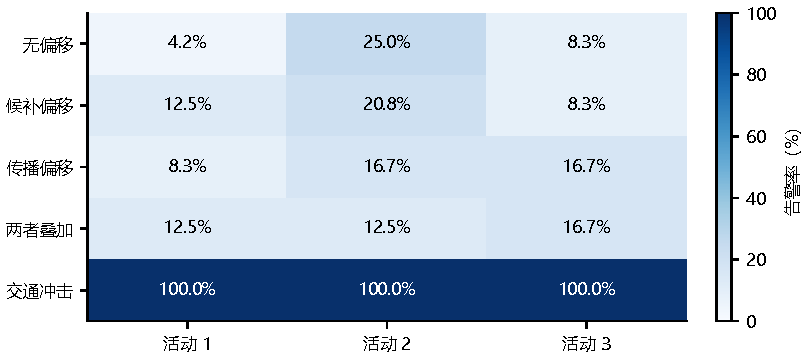
\includegraphics[width=.83\linewidth]{stress_alarms.pdf}
\caption{合成世界中 Full 的事后告警率。“无偏移”是误报对照。对强取消冲击的较好检出，与对候补、传播偏移的较弱检出同时存在。区间见表~\ref{tab:stress}。}
\label{fig:stress}
\end{figure}
原评测器要求认识方差较低且 RMSE 超过 $0.08$ 才告警，该诊断在补充实验的候补与传播扰动中从未触发。表~\ref{tab:stress_magnitude} 同时报告真值位移：部分模板的候补扰动很小，因此不能把不同偏移的漏检都解释为同等严重的失败。两种诊断均依赖已经实现的结果，不是事前预警。失配候选之间的一致意见，本身无法识别遗漏规则。

\subsection{RQ2：什么改善了证据效率，又是什么得到了加速？}
原开发 AUC 从 \InitialDev\ 降至 \FinalDev，在同一开发集自适应选择后下降 \DevReduction\%。冻结测试 AUC 为 \TestAUC。这是所选预测器在固定合成评测上的证据，不是相对外部最优方法的提升百分比。独立世界的宏平均结果是不同统计量，不能替换合并测试分数。

表~\ref{tab:acquisition_original} 与图~\ref{fig:curves} 上排给出原始比较。Full 的较低曲线包含进化校准的收益，其他取证器则从均匀相容权重出发。表~\ref{tab:acquisition_matched} 改为同先验比较后，表面的取证优势消失。同先验 Random 的宏平均 AUC 为 \MacroRandom，略低于 Full 的 \MacroFull。差异很小，近乎平坦的曲线说明初始集中的权重在很大程度上已决定预测。这些控制避免了把校准收益归到查询准则上。
\begin{table}[tbp]
\centering
\caption{原始对照：校准与取证策略同时变化。逐活动 AUC $\times10^3$，括号为 95\% 世界 bootstrap 区间；24 个独立世界，固定训练数据、证据与模板。}
\label{tab:acquisition_original}
\scriptsize
\setlength{\tabcolsep}{3pt}
\begin{tabular}{lrrr}
\toprule
方法 & 活动 1 & 活动 2 & 活动 3 \\
\midrule
Random & 17.82 [17.23, 18.39] & 19.03 [18.10, 20.01] & 14.96 [14.46, 15.44] \\
Entropy & 12.94 [12.27, 13.64] & 10.15 [9.21, 11.16] & 8.19 [7.32, 9.14] \\
ParamIG & 12.98 [12.34, 13.68] & 10.80 [10.06, 11.59] & 8.56 [7.50, 9.73] \\
Standard OED & 23.59 [22.32, 24.75] & 27.44 [24.79, 30.05] & 21.58 [19.34, 23.61] \\
Full & 4.19 [3.38, 5.07] & 10.85 [8.78, 12.85] & 6.15 [3.98, 8.65] \\
\bottomrule
\end{tabular}
\end{table}

\begin{table}[tbp]
\centering
\caption{同先验取证对照：所有方法采用进化先验。逐活动 AUC $\times10^3$，括号为 95\% 世界 bootstrap 区间；24 个独立世界，固定训练数据、证据与模板。}
\label{tab:acquisition_matched}
\scriptsize
\setlength{\tabcolsep}{3pt}
\begin{tabular}{lrrr}
\toprule
方法 & 活动 1 & 活动 2 & 活动 3 \\
\midrule
同先验 Random & 4.19 [3.38, 5.07] & 10.84 [8.77, 12.84] & 6.15 [3.98, 8.65] \\
同先验 Entropy & 4.19 [3.38, 5.07] & 10.85 [8.78, 12.85] & 6.15 [3.98, 8.65] \\
同先验 ParamIG & 4.19 [3.38, 5.07] & 10.85 [8.78, 12.85] & 6.15 [3.98, 8.65] \\
同先验 Standard OED & 4.19 [3.38, 5.07] & 10.85 [8.78, 12.85] & 6.15 [3.98, 8.65] \\
Full & 4.19 [3.38, 5.07] & 10.85 [8.78, 12.85] & 6.15 [3.98, 8.65] \\
\bottomrule
\end{tabular}
\end{table}

\begin{figure}[tbp]
\centering
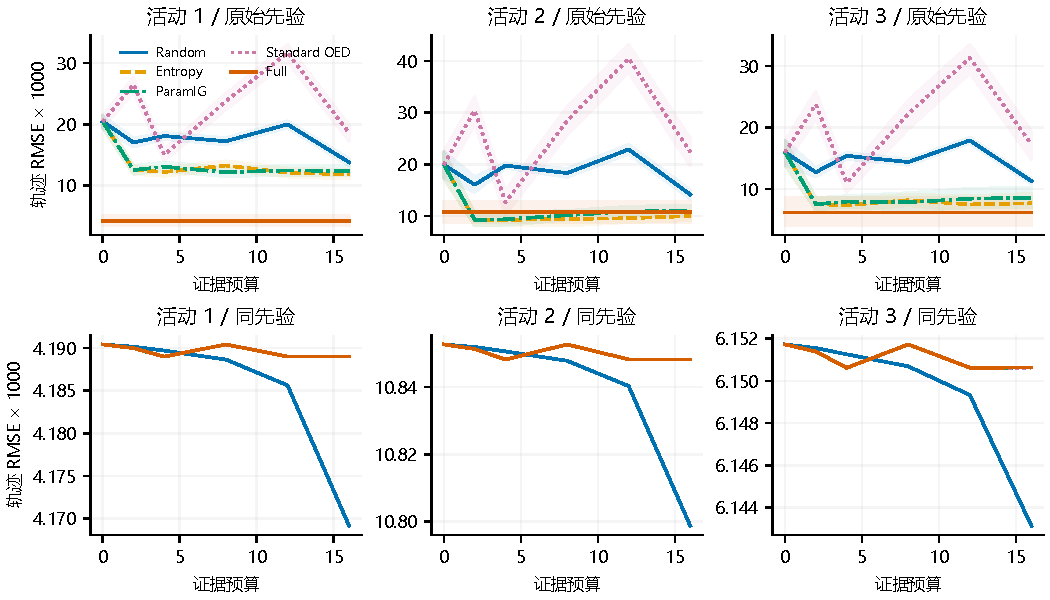
\includegraphics[width=\linewidth]{budget_curves.pdf}
\caption{逐活动展示的合成预算—轨迹误差曲线。上排为原校准策略，阴影是条件 95\% 世界 bootstrap 区间；下排全部使用进化先验，曲线几乎重合。下排保持绝对数值，但各图尺度不同，不能把其微小起伏与上排效应量直接作视觉比较。}
\label{fig:curves}
\end{figure}

\paragraph{评分微基准。}
使用相同候选、缓存预测、概率和成本，比较协方差评分与显式枚举二元结果。10 组 GPU 同步配对计时交替执行顺序。表~\ref{tab:timing} 报告冻结权重下 \FrozenSpeed\ 倍、均匀相容权重下 \UniformSpeed\ 倍的配对加速比中位数，以及最大评分残差。图~\ref{fig:evolution} 展示原始计时。参考实现是所提供的循环枚举版本；充分向量化的枚举器可以共享相当一部分计算。因此，这些测量证明的是局部实现优势，不是相对所有优化 OED 的普遍加速，也不是渐近复杂度改进。
\begin{table}[tbp]
\centering
\caption{10 次同步 GPU 配对计时，执行顺序交替。分别计算每一对的加速比再取中位数，因此不必等于两类时间中位数之比。}
\label{tab:timing}
\scriptsize
\setlength{\tabcolsep}{3pt}
\begin{tabular}{lrrrr}
\toprule
先验 & 协方差（毫秒） & 枚举（毫秒） & 配对加速比中位数 & 最大残差 \\
\midrule
冻结先验 & 0.773 & 178.17 & 217.95 & 9.08e-16 \\
均匀相容先验 & 0.747 & 191.85 & 275.16 & 1.38e-10 \\
\bottomrule
\end{tabular}
\end{table}

指定的冻结全量评测在 RTX 4060 Laptop GPU 上用时 \TestRuntime\ 秒，报告 PyTorch 峰值分配显存 \TestVRAM\ MB。它们仅对应缓存评测，不包含离线缓存生成和显卡驱动占用。开发试验约需 4 至 9 秒。小型缓存评测适合 8 GB 显存，但这不证明更大人群或更丰富机制库也能维持相同速度。

\subsection{RQ3：哪些改动经受住了受控消融？}
表~\ref{tab:ablations} 比较完整方法、四种移除设置以及匹配单点估计。移除组合目标或批量条件化，汇总结果不变。这与权重近乎单点的现象一致：若似然无法移动足够多的质量，改变查询选择也很难影响预测。取消共享会使结果变差，但该库使用逐活动独立参数排列，同时改变先验和假设空间。因此，这一结果描述的是相应实现，不是参数共享收益的纯因果估计。
\begin{table}[tbp]
\centering
\caption{冻结方法消融。星号表示同时改变了先验或单点选择目标。逐活动 AUC $\times10^3$，括号为 95\% 世界 bootstrap 区间；24 个独立世界，固定训练数据、证据与模板。}
\label{tab:ablations}
\scriptsize
\setlength{\tabcolsep}{3pt}
\begin{tabular}{lrrr}
\toprule
方法 & 活动 1 & 活动 2 & 活动 3 \\
\midrule
Full & 4.19 [3.38, 5.07] & 10.85 [8.78, 12.85] & 6.15 [3.98, 8.65] \\
取消参数共享* & 47.19 [45.23, 49.01] & 21.17 [18.72, 23.61] & 51.11 [48.60, 53.35] \\
移除组合目标 & 4.19 [3.38, 5.07] & 10.85 [8.78, 12.85] & 6.15 [3.98, 8.65] \\
原单点估计* & 5.42 [4.71, 6.08] & 7.54 [5.92, 9.35] & 7.37 [5.78, 8.95] \\
匹配 MAP & 4.19 [3.38, 5.07] & 10.85 [8.78, 12.85] & 6.15 [3.99, 8.65] \\
移除批量条件化 & 4.19 [3.38, 5.07] & 10.85 [8.78, 12.85] & 6.15 [3.98, 8.65] \\
\bottomrule
\end{tabular}
\end{table}


开发轨迹说明了集中如何形成。R1--R7 引入轨迹加权并逐步收窄核宽，R30 把历史平均误差换成最差活动误差。R38 再次收窄核宽，但接受的改善仅约 $10^{-7}$，不应作为性能跃升。R58 引入式~\eqref{eq:distance} 的噪声归一化，是后期最大的一次改善。由于每次接受的修改都会成为下一轮起点，这些顺序决策并不是彼此独立的消融。全部 60 个分数和决定见附录~\ref{app:trials}。

群体目标与过程预测也存在取舍：开发 Brier 从 \DevBrierStart\ 变差为 \DevBrierEnd，冻结测试 Brier 为 \TestBrier。冻结测试逐点覆盖率为 \TestCoverage\%，平均宽度为 \TestWidth。边际覆盖率较高，不等于机制得到识别，也不等于模型类外不确定性已校准。独立世界的不确定性表（表~\ref{tab:uncertainty}）分别报告认识与随机方差；在最终权重下，前者远小于后者。
\begin{figure}[tbp]
\centering
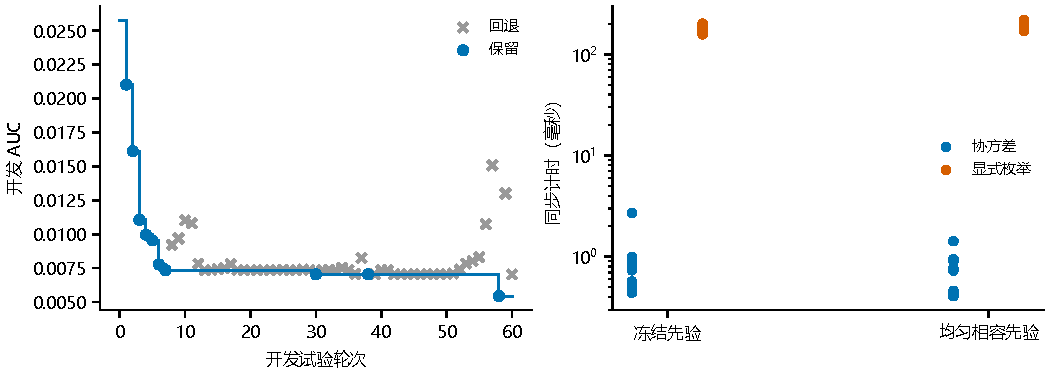
\includegraphics[width=\linewidth]{evolution_timing.pdf}
\caption{左：全部 60 个开发候选及保留分数轨迹，回退试验同样保留。右：每类先验的全部 10 组配对计时；对数坐标区分协方差与枚举成本，计时重复不作为独立活动样本。}
\label{fig:evolution}
\end{figure}

\subsection{第二阶段：非坍缩校准与同先验主动取证}
\label{sec:round2}
\paragraph{保留 V1，单独验证其失效原因。}
第~\ref{sec:method} 节及第 4.1--4.4 节报告原始 V1 研究。本节针对一个具体问题展开：如果校准后仍保留合理的候选机制，过程取证能否重新产生可测量的收益？我们保留 \texttt{eb641c2} 的代码、数据和原始结论，在独立分支预先固定新的压力场景、裁决护栏和 30 组开发配置。V1 与 V2 都在新场景上重新评测；不能把新旧基准的分数直接相减，再将差异全部归因于算法。

\paragraph{机制歧义的构造与统计单位。}
新配置采用 256 个智能体、8 个模拟种子、12 个时间步和 200 组候选机制。预先指定的两组机制为 $(a,b,d)=(.2,.95,.12)$ 与 $(.95,.2,.12)$，注意概率与参与概率的乘积相同。通过逆变换共同随机数耦合，二者生成相同的初始意图。历史活动分别启用候补或转发；组合活动同时启用候补通知触发的八邻居传播级联和强同时间冲突。这对机制的历史轨迹 RMSE 为 0.00000，组合探针及测试事件设计上的轨迹分歧为 0.28094。这是专门构造的交互压力测试，不是从真实行为数据拟合出的社会规律。

开发和测试分别使用 12 个与 24 个独立模拟世界。测试更换世界、过程审计和取证答案，事件设计仍与组合探针相同，因此它验证的是同一设计下的新世界复现，不是超出探针的新组合迁移。区间以整个世界为单位进行配对 bootstrap，保留世界内活动之间的依赖，逐活动另行报告。

\paragraph{校准公式与保留条件。}
在 V1 的历史相容支持集 $\mathcal C$ 上，设 $r_{etc}$ 为式~\eqref{eq:distance} 中的相对种子方差归一化项。V2 采用
\begin{align}
 E_m^{(2)}&=\frac{1}{2\sigma^2}\operatorname{mean}_{e,t,c}
 \frac{(\bar X_{metc}-H_{etc})^2}{r_{etc}}+\lambda\ell_m^{\mathrm{proc}},\\
 \ell_m^{\mathrm{proc}}&=-\frac{1}{|\mathcal O|}\sum_{j\in\mathcal O}
 [y_j\log p_{mj}+(1-y_j)\log(1-p_{mj})],\\
 w_{0m}^{(2)}&\propto\mathbf1[m\in\mathcal C]\exp(-E_m^{(2)}/T),\qquad
 T=\inf\{t\geq1:\,N_{\mathrm{eff}}(w_0(t))\geq8\}.
 \label{eq:v2-calibration}
\end{align}
实现中通过二分求解温度，并留出很小的数值余量。MCAR 缺失标签不贡献对数似然；意图记录中未观测的查看状态仍按 $p_{mj}=a_mb_m I_j$ 边缘化。支持集筛选条件不变。上述平均残差对应最终选中的 V2；搜索也包含最坏活动残差版本。Gibbs 温度可以解释为熵正则强度，但这里直接约束的有效机制数对应二阶 R\'enyi 熵，并非 Shannon 熵。

KEEP 必须同时满足：开发 AUC 比当前最优值下降超过 $10^{-8}$；初始有效机制数至少为 8；初始及预算 16 的过程审计 Brier 均不超过 .195；$R(0)-R(16)$ 的配对 95\% bootstrap 区间下界严格大于零；AUC 比同先验 Random 和 Entropy 均至少低 5\%；快速开发评测不超过 15 秒。每个版本内部的三种策略共用先验、证据池、成本、答案、缺失掩码和后验更新。给定所选证据 $D$，更新为
\begin{equation}
 w_m(D)\propto w_{0m}\exp\!\left\{\tau^{-1}
 \sum_{j\in D\cap\mathcal O}\log p_m(y_j)\right\}.
 \label{eq:v2-update}
\end{equation}
最终配置为 $\sigma=0.008$、$\lambda=8$、$\tau=0.5$，各时间步等权，批量大小为 2，并保留幻想分支条件化。假设答案分支与真实证据更新使用相同温度。由于 $\tau\ne1$，该更新属于广义贝叶斯；原协方差评分在此作为启发式排序使用，不能继续宣称它精确等于温度化后验的预期方差下降，也不增加次模性保证。

\paragraph{冻结后的对照结果。}
30 轮有效实验包含 3 次 KEEP、27 次 REVERT，没有运行失败，最优提交为 \texttt{0d094ec}。在同一新缓存上，V2 的初始有效机制数为 26.45，V1 为 1.01。表~\ref{tab:v2-overview} 给出同基准对照。V2 开发 AUC 为 0.07569，比同先验 Random 和 Entropy 分别低 27.5\% 和 43.2\%。读取测试真值前已冻结算法。测试 Full AUC 为 0.05776，95\% 区间为 [0.04948, 0.06688]；V1 为 0.14389，两者相差 59.9\%。V2 的误差从零证据时的 0.13319 降至预算 16 时的 0.03948，配对改善区间为 [0.08321, 0.10258]。初始和最终测试 Brier 分别为 0.18800 与 0.17438。初始 Brier 实际劣于 V1，只是两者均满足护栏；过程预测的改善发生在取证之后。
\begin{table}[tbp]
\centering\small
\setlength{\tabcolsep}{4pt}
\caption{第二阶段同一高分歧基准上的 V1/V2 对照。Brier 为预算 16 的独立过程审计误差。}\label{tab:v2-overview}
\begin{tabular}{llrrrrr}
\toprule
版本 & 划分 & 有效数 & AUC & B0 误差 & B16 误差 & Brier \\
\midrule
V1 & Dev & 1.01 & 0.14410 & 0.14606 & 0.14003 & 0.18197 \\
V2 & Dev & 26.45 & 0.07569 & 0.13327 & 0.04750 & 0.17416 \\
V1 & Test & 1.01 & 0.14389 & 0.14601 & 0.14007 & 0.18223 \\
V2 & Test & 26.45 & 0.05776 & 0.13319 & 0.03948 & 0.17438 \\
\bottomrule
\end{tabular}
\end{table}

\begin{table}[tbp]
\centering\small
\setlength{\tabcolsep}{4pt}
\caption{冻结测试：每个版本内严格共用先验和更新规则，区间按 24 个完整世界重采样。}\label{tab:v2-selectors}
\begin{tabular}{llrlr}
\toprule
版本 & 策略 & AUC & 95\% 区间 & Brier \\
\midrule
V1 & Full & 0.14389 & [0.14281, 0.14474] & 0.18223 \\
V1 & Random & 0.14589 & [0.14561, 0.14618] & 0.18291 \\
V1 & Entropy & 0.14601 & [0.14572, 0.14631] & 0.18296 \\
V1 & ParamIG & 0.14389 & [0.14281, 0.14474] & 0.18223 \\
V1 & Standard\_OED & 0.14392 & [0.14284, 0.14477] & 0.18223 \\
V2 & Full & 0.05776 & [0.04948, 0.06688] & 0.17438 \\
V2 & Random & 0.11579 & [0.10012, 0.13205] & 0.18523 \\
V2 & Entropy & 0.13319 & [0.13294, 0.13346] & 0.18800 \\
V2 & ParamIG & 0.05776 & [0.04948, 0.06688] & 0.17438 \\
V2 & Standard\_OED & 0.13315 & [0.13253, 0.13372] & 0.18810 \\
\bottomrule
\end{tabular}
\end{table}


测试集上，Full AUC 比同先验 Random 低 50.1\%，比同先验 Entropy 低 56.6\%；“基线减 Full”的配对 AUC 差值区间分别为 [0.03946, 0.07722] 与 [0.06633, 0.08376]。图~\ref{fig:v2-curves} 展示逐活动曲线，表~\ref{tab:v2-activities} 给出各活动的区间。然而 ParamIG 选择了相同记录，与 Full 完全持平，因此不能据此声称协方差取证优于参数信息增益。标准 OED 对照针对历史轨迹，表现较弱；它并不是经过优化的组合预测 OED 上界。
\begin{figure}[tbp]
\centering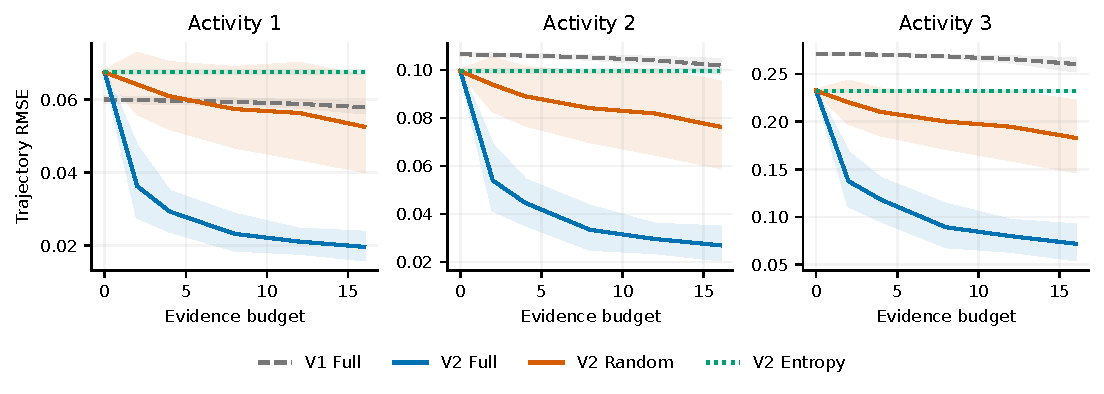
\includegraphics[width=\linewidth]{v2_budget_curves.pdf}
\caption{第二阶段冻结测试的逐活动曲线。阴影为逐点的 95\% 世界 bootstrap 区间。V2 的三种取证共用先验与更新；V1 使用原始校准。ParamIG 与 V2 Full 重合，为便于阅读省略。}
\label{fig:v2-curves}
\end{figure}
\begin{table}[tbp]
\centering\small
\setlength{\tabcolsep}{4pt}
\caption{逐活动的冻结测试结果。每个活动模板有 24 个独立世界实现；同一世界内的活动不视为独立。}\label{tab:v2-activities}
\begin{tabular}{llrll}
\toprule
版本 & 活动 & AUC & AUC 的 95\% 区间 & B0--B16 的 95\% 区间 \\
\midrule
V1 & 1 & 0.05911 & [0.05831, 0.05992] & [0.00109, 0.00358] \\
V1 & 2 & 0.10486 & [0.10382, 0.10567] & [0.00228, 0.00785] \\
V1 & 3 & 0.26770 & [0.26578, 0.26916] & [0.00519, 0.01849] \\
V2 & 1 & 0.02769 & [0.02393, 0.03177] & [0.04375, 0.05123] \\
V2 & 2 & 0.04041 & [0.03429, 0.04726] & [0.06506, 0.07858] \\
V2 & 3 & 0.10519 & [0.09004, 0.12190] & [0.14057, 0.17774] \\
\bottomrule
\end{tabular}
\end{table}


\paragraph{哪些变化有效，哪些结论仍不成立。}
30 组配置产生了 18 个不同的开发 AUC。在最终核宽下，将有效机制数下限从 8 提高到 24 没有改变权重，因为未触发温度提升时的有效机制数已超过 24。因此，护栏可以拒绝不合格候选，但最终配置的改善不能全部归因于护栏主动抬高温度。在核宽 .008、过程权重 8 不变时，将更新温度从 1 调到 .5，AUC 从 0.08193 降至 0.07569；温度 2 则恶化到 0.09056。这是可直接比较的温度实验。其他配置组同时改变核宽、过程权重或损失聚合方式，不能据此单独确定每个因素的因果贡献。移除批量幻想分支条件化后，匹配配置的选择记录和分数相同，这个证据池没有展示独立的批量去冗余收益。

证据池固定包含 24 条查看记录、40 条概率已知为 .5 的可用性记录，以及 96 条边缘化意图记录。最大熵策略将预算花在不可约的可用性随机性上，查看记录则能区分歧义的注意机制。这种设计使失效原因容易解释，也限定了结论：它有利于具有信息敏感性的选择策略，不能证明任意证据池上的普遍优势。测试增益大于开发增益，与固定历史条件下不同的取证答案有关，开发集仅含 12 个世界。当前证据支持“构造场景中恢复了主动取证价值”，尚不支持真实世界机制识别、新的未知规则告警保证或任何官方榜单成绩。


\section{讨论与相关工作}
\subsection{与校准和实验设计研究的关系}
\paragraph{不可识别情境下的校准。}
贝叶斯计算机模型校准区分参数不确定性与模型偏差 \citep{kennedy2001}。已有资格集合校准研究处理了多智能体模拟器的不可识别问题，并结合分布比较与贝叶斯优化 \citep{bai2022}。本文的经验过程／轨迹筛选更简单，不具有这些方法的统计检验解释。用于无似然推断的贝叶斯优化分配的是昂贵模拟器的评估次数 \citep{gutmann2016}，而本文在推演已经缓存后，分配的是过程记录的访问预算；两者对应不同的资源决策。因此，集合校准本身不是新颖性主张。本文着重把它与阶段取证机会、组合目标轨迹明确连接，并通过可审计实验研究这种连接何时失效。

\paragraph{预测导向取证。}
基于方差的主动学习已有长期研究 \citep{cohn1996}，贝叶斯实验设计则为取决于效用的数据获取提供了决策理论框架 \citep{chaloner1995}。目标导向 OED 关心预测量，而非全部参数不确定性 \citep{attia2018,zhong2026}。本文的协方差平方评分是有限机制、二元观测下的特例，采用方差效用而非预测信息增益。若各机制给某记录相同的概率，或该记录与探针预测不相关，即使行为熵很高，其取证价值也可能为零。实际关键在于阶段似然是否有效、探针目标分布是否合适、数值支持是否保留，以及计算能否复用。当前证据对计算复用的支持最明确。

\paragraph{社会模拟系统。}
CALM 将校准后的随机选择用于基于活动的出行模拟 \citep{cheng2026}，针对的是具体真实移动场景，而非本文的有限过程记录获取问题。SocioVerse2 为社会系统建立纵向模拟与研究循环 \citep{zhang2026}；Large Population Models 强调群体规模的行为与互动 \citep{chopra2025}。这些系统支持在机制、观测和集体结果之间建立可复用接口的研究方向，但并非本文已经运行的实证基线。给适配器起一个基准名称，也不等于复现了该基准的评测。提案中从宏观观测学习个体动态的更广泛目标，在 macro2mind 中也有所体现 \citep{macro2mind2026}；本文没有实现或比较这一模型。真实领域比较仍需要相容的观测机会、有授权的数据，以及具名且冻结的评分协议。

\subsection{适用范围、边界条件与失效模式}
\label{sec:boundaries}
\paragraph{权重集中会消除取证所依赖的信号。}
当 $w$ 趋近单点质量时，对每条记录均有 $\Cov_w(p_r,Z)\to0$，因而 $A_r(w)\to0$。所以，较大的硬相容集合不足以保证保留认识不确定性。较小核宽与有限精度 softmax 共同限制了有效支持；后验更新无法恢复恰好为零的候选质量。实测未发现取证收益，与这一极限行为一致，但要定量证明其贡献，还需超出本冻结研究的受控干预。

\paragraph{为什么一些看似合理的改动失败了。}
R8--R9 和 R36--R37 的较宽核被回退：在当前开发目标下，给更多候选保留质量增加了预测误差。R14--R17、R50--R53 混入均匀权重，也没有改善目标。这些结果区分了数值多样性与准确不确定性，并不证明多样化集合通常更差。R10--R11 将温度降到 $0.05$ 和 $0.1$、加强证据似然后，结果变差，这与有限机制库失配时少量噪声二元证据的过度影响相符。混合分布已经高度集中后，后续温度变化只带来极小差别。

R18--R23 加入过程 Brier 能量，所选行为几乎未变；R24--R29 调整通道权重，没有取得超过接受阈值的改善。R31--R35 的最差通道、绝对误差、Huber、截尾与后半程损失也未提高分数。这些损失体现不同的拟合观念，没有哪一个是普遍有效的稳健修正。R42--R45 重缩放探针坐标后 AUC 完全相同，因此不能把这些已回退的构想写成最终方法的创新。R54--R57 的种子边缘化核表现更差，但同时改变了校准构造与核尺度，不能据此断言随机性建模有害。最后，R59--R60 提高方差底值，使 R58 的收益消失；这种正则敏感性是一项限制，而不是所选参数能迁移到新领域的证据。

\paragraph{批量条件化不蕴含次模性。}
自适应次模保证需要边际收益递减性质 \citep{golovin2011}，本文目标一般不满足它。考虑以两个独立公平二元变量 $(U,V)$ 表示机制，目标 $Z=U\oplus V$ 是两者的异或，两个无噪声查询分别揭示 $U$ 和 $V$。任一查询单独出现时，目标方差都不变；两个一起则完全确定 $Z$。即使给定机制后查询是确定的、因而条件独立，第二个查询的边际价值仍在第一个查询后增加，违反收益递减。这个解析反例说明，精确假设分支期望应称为贪心条件化取证，不能赋予通用近似保证。

\paragraph{预测一致与任意程度的模型失配可以同时存在。}
假设所有候选预测 $z_0$，而一个遗漏的环境规则使现实变成 $z_0+\Delta$。所有认识协方差与取证评分都为零，但均方误差为 $\|\Delta\|^2/D$。方差缩减恒等式在模型内部依然成立，却无法发现候选类中根本不存在的机制；较宽的随机区间还可能掩盖弱偏移。事后残差检查提供另一种证据来源，但本研究中的阈值既没有校准的误报控制，也没有事前预警保证。扩充候选与显式偏差建模是可能的改进方向，而非已经实现的成功结果。

\paragraph{当前证据支持什么，不支持什么。}
同一个开发划分用于选择 60 个候选，只报告最优分数而不披露搜索历史，会夸大验证力度。测试评测与独立世界扩展增强了可复现性，但仍固定活动模板、训练数据、证据和小型有限机制库。文中的任何置信区间都没有覆盖真实人群不确定性或搜索过程本身的不确定性。第~\ref{sec:round2} 节使用新的查询群体和封存测试集，部分回应了这一问题。后续仍需改变事件设计、历史数据和证据池，加入同先验且优化实现的 OED，检验非坍缩取证收益能否超出本次构造的压力场景。还应把参数共享与先验变化分开，在使用真实行为记录前验证观测模型。

\subsection{结论}
本文明确并实现了一个计算成本较低的预算化过程取证闭环，支持完整轨迹预测和分解的不确定性。最重要的经验发现是：成功的群体校准可能消除主动取证赖以发挥作用的机制分歧。冻结实现改善了合成轨迹预测，并加速了参考评分计算，但 V1 的匹配对照没有建立主动取证或保留集合的优势。独立的 V2 压力测试展示了相对同先验 Random 和 Entropy 的取证收益，同时与 ParamIG 持平；其刻意设置的无关高熵记录和未生效的批量消融限定了结论范围。将这种区别如实作为结果，比未经支持地宣称机制已被识别或超越外部基准，更有助于为组合式社会模拟建立可靠研究基础。

\bibliographystyle{plainnat}
\bibliography{references}
\clearpage
\appendix
\section{补充结果与审计记录}
\label{app:results}
以下各表与正文使用同一批封存结果，并非新增调参实验。表~\ref{tab:golden} 保留原评测器的合并指标，其他活动表采用独立世界重复。明确这一区别，可以避免将聚合方式的改变误认为方法性能的改变。参考文献保留原文题名与作者，便于检索。
\begin{table}[H]
\centering
\caption{原冻结测试缓存的描述性结果。Random 对三次查询重复取平均；这些相互影响的活动不是独立重复样本。}
\label{tab:golden}
\scriptsize
\setlength{\tabcolsep}{3pt}
\begin{tabular}{lrrrrr}
\toprule
方法 & 合并 AUC & Brier & NLL & 覆盖率 & 宽度 \\
\midrule
Random & 0.017980 & 0.1957 & 0.5775 & 1.0000 & 0.0666 \\
Entropy & 0.011052 & 0.1862 & 0.5572 & 1.0000 & 0.0691 \\
ParamIG & 0.011017 & 0.1860 & 0.5618 & 1.0000 & 0.0679 \\
Standard OED & 0.025494 & 0.2086 & 0.6021 & 1.0000 & 0.0666 \\
Full & 0.006916 & 0.2459 & 0.6811 & 0.9792 & 0.0304 \\
简单统计模型 & 0.023584 & 0.3026 & 0.8458 & 0.8125 & 0.0318 \\
未校准模型 & 0.017490 & 0.2144 & 0.6139 & 1.0000 & 0.0896 \\
仅过程校准 & 0.019877 & 0.2238 & 0.6328 & 1.0000 & 0.0769 \\
仅轨迹校准 & 0.018181 & 0.2202 & 0.6253 & 1.0000 & 0.0804 \\
被动 V1 & 0.019877 & 0.2238 & 0.6328 & 1.0000 & 0.0769 \\
取消参数共享* & 0.051271 & 0.2050 & 0.6108 & 0.6146 & 0.0360 \\
移除组合目标 & 0.006916 & 0.2459 & 0.6811 & 0.9792 & 0.0304 \\
原单点估计* & 0.008321 & 0.2513 & 0.7070 & 0.9479 & 0.0291 \\
\bottomrule
\end{tabular}
\end{table}

\begin{table}[H]
\centering
\caption{被动校准基线，不获取额外证据。逐活动 AUC $\times10^3$，括号为 95\% 世界 bootstrap 区间；24 个独立世界，固定训练数据、证据与模板。}
\label{tab:calibration}
\scriptsize
\setlength{\tabcolsep}{3pt}
\begin{tabular}{lrrr}
\toprule
方法 & 活动 1 & 活动 2 & 活动 3 \\
\midrule
简单统计模型 & 24.05 [23.81, 24.30] & 32.30 [30.39, 34.18] & 18.84 [18.07, 19.77] \\
未校准模型 & 19.99 [19.34, 20.63] & 17.08 [15.25, 18.87] & 13.81 [12.79, 14.89] \\
仅过程校准 & 20.43 [19.38, 21.40] & 19.94 [17.30, 22.45] & 15.96 [13.85, 17.89] \\
仅轨迹校准 & 19.56 [18.65, 20.40] & 17.66 [15.15, 20.03] & 14.28 [12.53, 15.93] \\
被动 V1 & 20.43 [19.38, 21.40] & 19.94 [17.30, 22.45] & 15.96 [13.85, 17.89] \\
\bottomrule
\end{tabular}
\end{table}

\begin{table}[H]
\centering
\caption{对照减 Full 的配对活动 AUC 差值 $\times10^6$，附 95\% 世界 bootstrap 区间。正值有利于 Full；微小差值不一定具有实际意义。}
\label{tab:paired}
\scriptsize
\setlength{\tabcolsep}{3pt}
\begin{tabular}{lrrr}
\toprule
对照减 Full & 活动 1 & 活动 2 & 活动 3 \\
\midrule
匹配 MAP & 1.19 [0.62, 1.84] & 3.72 [2.22, 5.21] & 0.92 [-0.18, 2.07] \\
同先验 Random & -3.61 [-5.60, -1.70] & -8.86 [-13.65, -3.83] & -1.38 [-5.02, 2.14] \\
移除组合目标 & 0.00 [0.00, 0.00] & 0.00 [0.00, 0.00] & 0.00 [0.00, 0.00] \\
移除批量条件化 & 0.00 [0.00, 0.00] & 0.00 [0.00, 0.00] & 0.00 [0.00, 0.00] \\
\bottomrule
\end{tabular}
\end{table}

\begin{table}[H]
\centering
\caption{最终预算下的不确定性均值与 95\% 世界 bootstrap 区间。覆盖率对应逐点 90\% 预测区间。}
\label{tab:uncertainty}
\scriptsize
\setlength{\tabcolsep}{3pt}
\begin{tabular}{lrrr}
\toprule
量 & 活动 1 & 活动 2 & 活动 3 \\
\midrule
覆盖率（百分比） & 94.0 [91.9, 95.9] & 90.8 [87.9, 93.7] & 92.5 [89.0, 95.4] \\
区间宽度（比例） & 0.0167 [0.0135, 0.0202] & 0.0349 [0.0313, 0.0387] & 0.0304 [0.0277, 0.0333] \\
认识方差 $\times10^8$ & 3.41 [2.65, 4.22] & 9.71 [6.72, 13.12] & 4.45 [3.01, 6.14] \\
随机方差 $\times10^4$ & 0.91 [0.69, 1.14] & 3.04 [2.48, 3.69] & 2.42 [2.05, 2.80] \\
\bottomrule
\end{tabular}
\end{table}

\begin{table}[H]
\centering
\caption{相对于无偏移世界的真实轨迹位移，RMSE $\times10^3$。单独报告偏移强度，以区分扰动很弱与检测不敏感。}
\label{tab:stress_magnitude}
\scriptsize
\setlength{\tabcolsep}{3pt}
\begin{tabular}{lrrr}
\toprule
真值规则 & 活动 1 & 活动 2 & 活动 3 \\
\midrule
无偏移 & 0.00 [0.00, 0.00] & 0.00 [0.00, 0.00] & 0.00 [0.00, 0.00] \\
候补偏移 & 3.55 [3.18, 3.93] & 0.61 [0.28, 0.97] & 0.38 [0.18, 0.61] \\
传播偏移 & 7.92 [7.35, 8.54] & 10.16 [9.17, 11.16] & 19.64 [18.42, 20.70] \\
两者叠加 & 7.37 [6.75, 8.07] & 10.15 [9.17, 11.15] & 19.21 [17.98, 20.30] \\
交通冲击 & 59.52 [58.46, 60.48] & 74.78 [72.55, 76.86] & 53.31 [51.58, 54.89] \\
\bottomrule
\end{tabular}
\end{table}

\FloatBarrier
\section{复现方式与证据来源}
\label{app:reproduction}
冻结算法对应提交 \texttt{eb641c2}，其 SHA-256 记录在机器可读的制品清单中。图表生成器首先核对算法哈希，再读取指定的冻结评测、24 世界补充实验、候选审计记录和研究循环汇总。根目录下其余 JSON 结果均登记来源与哈希，作为历史实验或复现记录保留，没有按测试成绩择优选取。候选审计按运行标识关联“评测行”和“决策行”，并核对 Git 源码。因此，搜索预算是 60 个不同候选，而不是账本总行数。

研究包将环境准备、固定评测器、唯一可演化算法文件与搜索控制器分开。撰写本文没有修改这些组件。原缓存把标签保存在同一本地进程可访问的位置；源码核验与接口约定提供的是可审计性，不是能够抵御越权访问的安全保留集。涉及敏感观测时，仍需独立且有权限控制的评测服务。

英文图表可在研究根目录运行 \texttt{python paper/generate\_artifacts.py} 重建，英文 PDF 由 \texttt{python paper/build.py} 编译。中文版使用 \texttt{python paper/generate\_zh\_assets.py} 生成中文图表，再以 \texttt{python paper/build\_zh.py} 调用 XeLaTeX 与 BibTeX 编译。这些操作均不运行新的研究实验。根目录下的科研复现脚本则用于重新执行封存合成实验，两种流程相互独立。缓存评测不计离线模拟成本；表~\ref{tab:timing} 的评分计时还不包括加载、校准、后验预测和绘图。

本研究没有招募真实参与者，也没有使用真实学生记录。可执行模型描述的是构造出的资源参与过程，其参数不能解读为个人心理特征的估计。SocioVerse 与 SocialSim 的对接材料属于接口准备，不是外部有效性的证据，也不等于正式榜单提交。本中文稿用于审阅，与英文稿使用同一份数据、公式与结论。

\section{完整开发决策}
\label{app:trials}
表~\ref{tab:alltrials} 按时间顺序报告全部接受与回退的候选。“回退”也包括数值上几乎无差别、或改善未达到预先规定阈值的情况，并不总意味着明显退化。假设、完整源码哈希和候选文件保存在仓库演化审计中。这些观察解释了最终实现的形成过程，但不能替代在新数据上对相应数学选择进行独立比较。
\footnotesize
\begin{longtable}{rrrll}
\caption{全部 60 个经审计的候选。开发分数来自自适应选择，不是独立验证。}\label{tab:alltrials}\\
\toprule 轮次 & 开发 AUC & 父版本 AUC & 决定 & 提交 \\ \midrule\endfirsthead
\toprule 轮次 & 开发 AUC & 父版本 AUC & 决定 & 提交 \\ \midrule\endhead
1 & 0.02103133 & 0.02579135 & 保留 & \texttt{9004e27} \\
2 & 0.01612103 & 0.02103133 & 保留 & \texttt{6bb9ddb} \\
3 & 0.01106276 & 0.01612103 & 保留 & \texttt{73386c1} \\
4 & 0.00996100 & 0.01106276 & 保留 & \texttt{728d215} \\
5 & 0.00954380 & 0.00996100 & 保留 & \texttt{ba8b306} \\
6 & 0.00776780 & 0.00954380 & 保留 & \texttt{d5e58c8} \\
7 & 0.00734499 & 0.00776780 & 保留 & \texttt{ef86a46} \\
8 & 0.00921580 & 0.00734499 & 回退 & \texttt{73f16c4} \\
9 & 0.00969213 & 0.00734499 & 回退 & \texttt{478719a} \\
10 & 0.01102639 & 0.00734499 & 回退 & \texttt{05f5dcf} \\
11 & 0.01080275 & 0.00734499 & 回退 & \texttt{b4c4fca} \\
12 & 0.00780723 & 0.00734499 & 回退 & \texttt{3088266} \\
13 & 0.00734522 & 0.00734499 & 回退 & \texttt{b4fe2a0} \\
14 & 0.00735953 & 0.00734499 & 回退 & \texttt{3df239c} \\
15 & 0.00741803 & 0.00734499 & 回退 & \texttt{25afcf5} \\
16 & 0.00749185 & 0.00734499 & 回退 & \texttt{4b1e757} \\
17 & 0.00779464 & 0.00734499 & 回退 & \texttt{bff1fc7} \\
18 & 0.00734499 & 0.00734499 & 回退 & \texttt{ff4fbbf} \\
19 & 0.00734499 & 0.00734499 & 回退 & \texttt{dbba10b} \\
20 & 0.00734499 & 0.00734499 & 回退 & \texttt{e09f641} \\
21 & 0.00734499 & 0.00734499 & 回退 & \texttt{35d2997} \\
22 & 0.00734499 & 0.00734499 & 回退 & \texttt{99e2128} \\
23 & 0.00734499 & 0.00734499 & 回退 & \texttt{0a72bd0} \\
24 & 0.00734499 & 0.00734499 & 回退 & \texttt{2721c24} \\
25 & 0.00737358 & 0.00734499 & 回退 & \texttt{6ebab02} \\
26 & 0.00734499 & 0.00734499 & 回退 & \texttt{0cae7ed} \\
27 & 0.00734532 & 0.00734499 & 回退 & \texttt{7292291} \\
28 & 0.00739139 & 0.00734499 & 回退 & \texttt{037df88} \\
29 & 0.00734499 & 0.00734499 & 回退 & \texttt{d83f2e1} \\
30 & 0.00704311 & 0.00734499 & 保留 & \texttt{98d6fb0} \\
31 & 0.00734499 & 0.00704311 & 回退 & \texttt{bc4d425} \\
32 & 0.00738014 & 0.00704311 & 回退 & \texttt{55a1b8f} \\
33 & 0.00734523 & 0.00704311 & 回退 & \texttt{f29e090} \\
34 & 0.00751265 & 0.00704311 & 回退 & \texttt{07fe993} \\
35 & 0.00734499 & 0.00704311 & 回退 & \texttt{4e8b0ca} \\
36 & 0.00706689 & 0.00704311 & 回退 & \texttt{f929916} \\
37 & 0.00823951 & 0.00704311 & 回退 & \texttt{f7fee7e} \\
38 & 0.00704303 & 0.00704311 & 保留 & \texttt{6a44dfc} \\
39 & 0.00704303 & 0.00704303 & 回退 & \texttt{9007fd6} \\
40 & 0.00734499 & 0.00704303 & 回退 & \texttt{4612d6b} \\
41 & 0.00734499 & 0.00704303 & 回退 & \texttt{7702d9c} \\
42 & 0.00704303 & 0.00704303 & 回退 & \texttt{6ff50b7} \\
43 & 0.00704303 & 0.00704303 & 回退 & \texttt{eb9bd17} \\
44 & 0.00704303 & 0.00704303 & 回退 & \texttt{8361b7a} \\
45 & 0.00704303 & 0.00704303 & 回退 & \texttt{be36314} \\
46 & 0.00704304 & 0.00704303 & 回退 & \texttt{871658d} \\
47 & 0.00704303 & 0.00704303 & 回退 & \texttt{f7077c6} \\
48 & 0.00704303 & 0.00704303 & 回退 & \texttt{320da5d} \\
49 & 0.00704303 & 0.00704303 & 回退 & \texttt{945ecb9} \\
50 & 0.00704964 & 0.00704303 & 回退 & \texttt{34ebfd4} \\
51 & 0.00711002 & 0.00704303 & 回退 & \texttt{72363f1} \\
52 & 0.00739650 & 0.00704303 & 回退 & \texttt{39cf814} \\
53 & 0.00782675 & 0.00704303 & 回退 & \texttt{307cd3d} \\
54 & 0.00802215 & 0.00704303 & 回退 & \texttt{c34f927} \\
55 & 0.00829448 & 0.00704303 & 回退 & \texttt{a7e246c} \\
56 & 0.01073823 & 0.00704303 & 回退 & \texttt{3c56dc0} \\
57 & 0.01507502 & 0.00704303 & 回退 & \texttt{b4ee347} \\
58 & 0.00543199 & 0.00704303 & 保留 & \texttt{eb641c2} \\
59 & 0.01300248 & 0.00543199 & 回退 & \texttt{1b4c940} \\
60 & 0.00704303 & 0.00543199 & 回退 & \texttt{135f671} \\
\bottomrule
\end{longtable}

\end{document}
